\documentclass{standalone}
\usepackage{tikz}
\usetikzlibrary{patterns, positioning}
\usepackage[sfdefault]{ClearSans} %% option 'sfdefault' activates Clear Sans as the default text font
\usepackage[T1]{fontenc}

\begin{document}
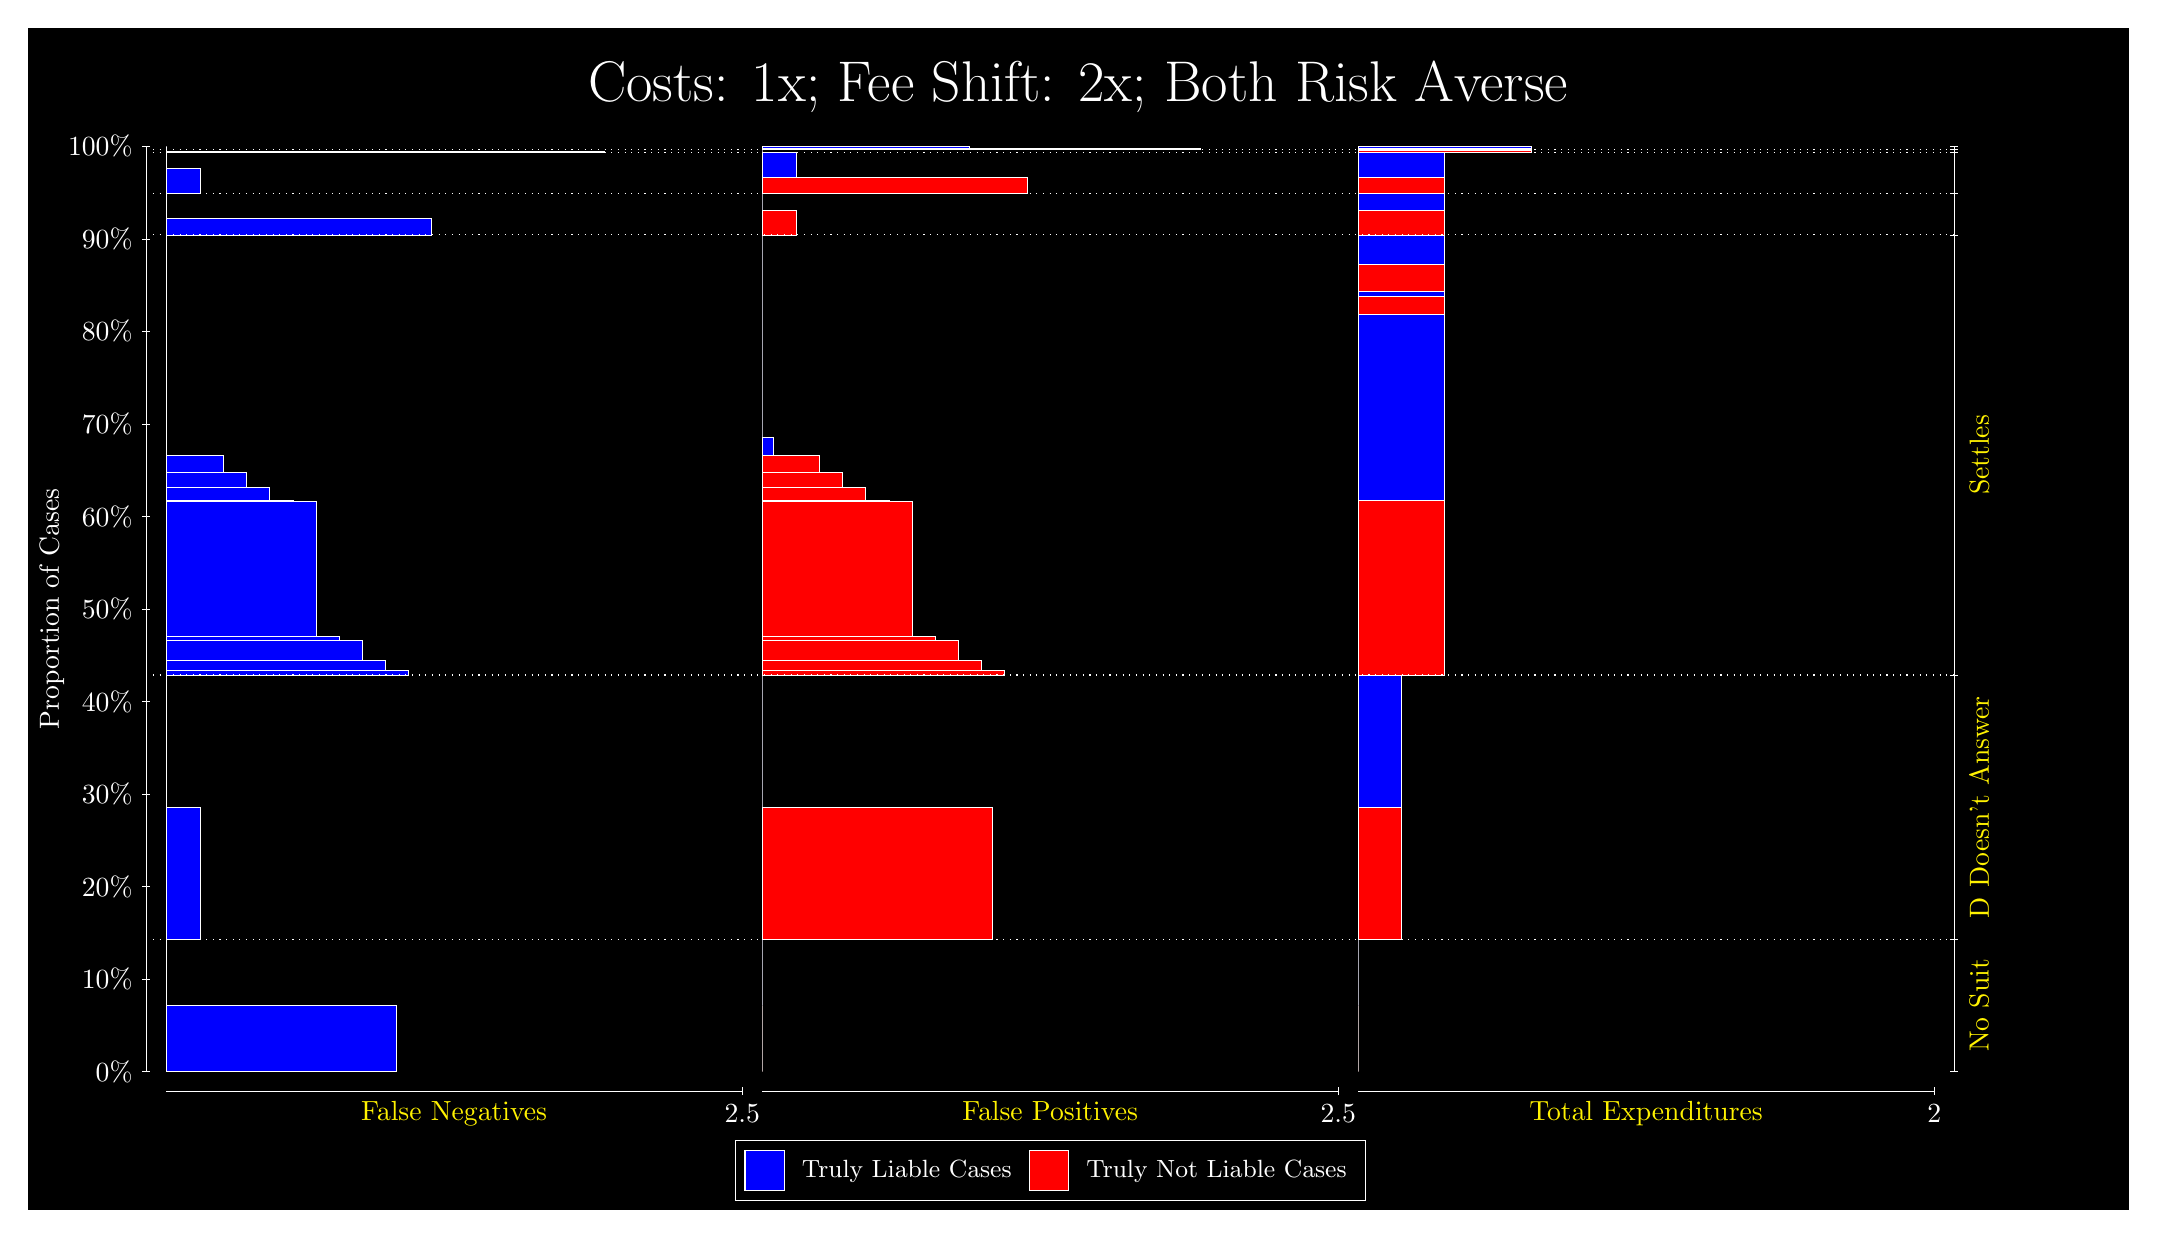
\begin{tikzpicture}
\draw[fill=black] (0,0) rectangle (26.667,15);
\draw[text=white] (0,13.5) rectangle (26.667,15) node[midway] {\huge Costs: 1x; Fee Shift: 2x; Both Risk Averse};
\draw[white, very thin] (1.5,1.75) -- (1.5,13.5);
\node[rotate=90, text=white, anchor=center] at (0.3, 7.625) {Proportion of Cases};
\draw[white, very thin] (1.45,1.75) -- (1.55,1.75);
\node[text=white, anchor=east] at (1.45, 1.75) {0\%};
\draw[white, very thin] (1.45,2.925) -- (1.55,2.925);
\node[text=white, anchor=east] at (1.45, 2.925) {10\%};
\draw[white, very thin] (1.45,4.1) -- (1.55,4.1);
\node[text=white, anchor=east] at (1.45, 4.1) {20\%};
\draw[white, very thin] (1.45,5.275) -- (1.55,5.275);
\node[text=white, anchor=east] at (1.45, 5.275) {30\%};
\draw[white, very thin] (1.45,6.45) -- (1.55,6.45);
\node[text=white, anchor=east] at (1.45, 6.45) {40\%};
\draw[white, very thin] (1.45,7.625) -- (1.55,7.625);
\node[text=white, anchor=east] at (1.45, 7.625) {50\%};
\draw[white, very thin] (1.45,8.8) -- (1.55,8.8);
\node[text=white, anchor=east] at (1.45, 8.8) {60\%};
\draw[white, very thin] (1.45,9.975) -- (1.55,9.975);
\node[text=white, anchor=east] at (1.45, 9.975) {70\%};
\draw[white, very thin] (1.45,11.15) -- (1.55,11.15);
\node[text=white, anchor=east] at (1.45, 11.15) {80\%};
\draw[white, very thin] (1.45,12.325) -- (1.55,12.325);
\node[text=white, anchor=east] at (1.45, 12.325) {90\%};
\draw[white, very thin] (1.45,13.5) -- (1.55,13.5);
\node[text=white, anchor=east] at (1.45, 13.5) {100\%};

\draw[white, very thin] (24.457,1.75) -- (24.457,13.5);
\draw[white, very thin] (24.407,1.75) -- (24.507,1.75);
\node[anchor=west] at (24.407, 1.75) {};
\draw[white, very thin] (24.407,3.4286) -- (24.507,3.4286);
\node[anchor=west] at (24.407, 3.4286) {};
\draw[white, very thin] (24.407,6.7857) -- (24.507,6.7857);
\node[anchor=west] at (24.407, 6.7857) {};
\draw[white, very thin] (24.407,12.376) -- (24.507,12.376);
\node[anchor=west] at (24.407, 12.376) {};
\draw[white, very thin] (24.407,12.9) -- (24.507,12.9);
\node[anchor=west] at (24.407, 12.9) {};
\draw[white, very thin] (24.407,13.424) -- (24.507,13.424);
\node[anchor=west] at (24.407, 13.424) {};
\draw[white, very thin] (24.407,13.462) -- (24.507,13.462);
\node[anchor=west] at (24.407, 13.462) {};
\draw[white, very thin] (24.407,13.5) -- (24.507,13.5);
\node[anchor=west] at (24.407, 13.5) {};

\draw[white, very thin, fill=blue] (1.75,1.75) rectangle (4.6775,2.5893);
\draw[white, very thin, fill=red] (1.75,2.5893) rectangle (1.75,3.4286);
\draw[white, very thin, fill=blue] (1.75,3.4286) rectangle (2.1891,5.1071);
\draw[white, very thin, fill=red] (1.75,5.1071) rectangle (1.75,6.7857);
\draw[white, very thin, fill=blue] (1.75,6.7857) rectangle (4.8239,6.8473);
\draw[white, very thin, fill=blue] (1.75,6.8473) rectangle (4.5312,6.972);
\draw[white, very thin, fill=blue] (1.75,6.972) rectangle (4.2384,7.2208);
\draw[white, very thin, fill=blue] (1.75,7.2208) rectangle (3.9457,7.2787);
\draw[white, very thin, fill=blue] (1.75,7.2787) rectangle (3.6529,8.9897);
\draw[white, very thin, fill=blue] (1.75,8.9897) rectangle (3.3602,9.0089);
\draw[white, very thin, fill=blue] (1.75,9.0089) rectangle (3.0674,9.168);
\draw[white, very thin, fill=blue] (1.75,9.168) rectangle (2.7746,9.3559);
\draw[white, very thin, fill=blue] (1.75,9.3559) rectangle (2.4819,9.5807);
\draw[white, very thin, fill=red] (1.75,9.5807) rectangle (1.75,12.376);
\draw[white, very thin, fill=blue] (1.75,12.376) rectangle (5.1167,12.581);
\draw[white, very thin, fill=red] (1.75,12.581) rectangle (1.75,12.9);
\draw[white, very thin, fill=blue] (1.75,12.9) rectangle (2.1891,13.218);
\draw[white, very thin, fill=red] (1.75,13.218) rectangle (1.75,13.424);
\draw[white, very thin, fill=blue] (1.75,13.424) rectangle (7.3123,13.438);
\draw[white, very thin, fill=red] (1.75,13.438) rectangle (1.75,13.462);
\draw[white, very thin, fill=red] (1.75,13.462) rectangle (1.75,13.476);
\draw[white, very thin, fill=blue] (1.75,13.476) rectangle (1.75,13.5);
\draw[white, very thin, fill=red] (9.3189,1.75) rectangle (9.3189,2.5893);
\draw[white, very thin, fill=blue] (9.3189,2.5893) rectangle (9.3189,3.4286);
\draw[white, very thin, fill=red] (9.3189,3.4286) rectangle (12.246,5.1071);
\draw[white, very thin, fill=blue] (9.3189,5.1071) rectangle (9.3189,6.7857);
\draw[white, very thin, fill=red] (9.3189,6.7857) rectangle (12.393,6.8473);
\draw[white, very thin, fill=red] (9.3189,6.8473) rectangle (12.1,6.972);
\draw[white, very thin, fill=red] (9.3189,6.972) rectangle (11.807,7.2208);
\draw[white, very thin, fill=red] (9.3189,7.2208) rectangle (11.515,7.2787);
\draw[white, very thin, fill=red] (9.3189,7.2787) rectangle (11.222,8.9896);
\draw[white, very thin, fill=red] (9.3189,8.9896) rectangle (10.929,9.0088);
\draw[white, very thin, fill=red] (9.3189,9.0088) rectangle (10.636,9.168);
\draw[white, very thin, fill=red] (9.3189,9.168) rectangle (10.344,9.3559);
\draw[white, very thin, fill=red] (9.3189,9.3559) rectangle (10.051,9.5806);
\draw[white, very thin, fill=blue] (9.3189,9.5806) rectangle (9.4652,9.8054);
\draw[white, very thin, fill=blue] (9.3189,9.8054) rectangle (9.3189,12.376);
\draw[white, very thin, fill=red] (9.3189,12.376) rectangle (9.758,12.694);
\draw[white, very thin, fill=blue] (9.3189,12.694) rectangle (9.3189,12.9);
\draw[white, very thin, fill=red] (9.3189,12.9) rectangle (12.686,13.106);
\draw[white, very thin, fill=blue] (9.3189,13.106) rectangle (9.758,13.424);
\draw[white, very thin, fill=red] (9.3189,13.424) rectangle (9.3189,13.448);
\draw[white, very thin, fill=blue] (9.3189,13.448) rectangle (9.3189,13.462);
\draw[white, very thin, fill=red] (9.3189,13.462) rectangle (14.881,13.476);
\draw[white, very thin, fill=blue] (9.3189,13.476) rectangle (11.954,13.5);
\draw[white, very thin, fill=red] (16.888,1.75) rectangle (16.888,2.5893);
\draw[white, very thin, fill=blue] (16.888,2.5893) rectangle (16.888,3.4286);
\draw[white, very thin, fill=red] (16.888,3.4286) rectangle (17.437,5.1071);
\draw[white, very thin, fill=blue] (16.888,5.1071) rectangle (17.437,6.7857);
\draw[white, very thin, fill=red] (16.888,6.7857) rectangle (17.986,9.0088);
\draw[white, very thin, fill=blue] (16.888,9.0088) rectangle (17.986,11.369);
\draw[white, very thin, fill=red] (16.888,11.369) rectangle (17.986,11.593);
\draw[white, very thin, fill=blue] (16.888,11.593) rectangle (17.986,11.655);
\draw[white, very thin, fill=red] (16.888,11.655) rectangle (17.986,12.002);
\draw[white, very thin, fill=blue] (16.888,12.002) rectangle (17.986,12.376);
\draw[white, very thin, fill=red] (16.888,12.376) rectangle (17.986,12.694);
\draw[white, very thin, fill=blue] (16.888,12.694) rectangle (17.986,12.9);
\draw[white, very thin, fill=red] (16.888,12.9) rectangle (17.986,13.106);
\draw[white, very thin, fill=blue] (16.888,13.106) rectangle (17.986,13.424);
\draw[white, very thin, fill=red] (16.888,13.424) rectangle (19.083,13.448);
\draw[white, very thin, fill=blue] (16.888,13.448) rectangle (19.083,13.462);
\draw[white, very thin, fill=red] (16.888,13.462) rectangle (19.083,13.476);
\draw[white, very thin, fill=blue] (16.888,13.476) rectangle (19.083,13.5);
\draw[white, dotted] (1.5,3.4286) -- (24.457,3.4286);
\draw[white, dotted] (1.5,6.7857) -- (24.457,6.7857);
\draw[white, dotted] (1.5,12.376) -- (24.457,12.376);
\draw[white, dotted] (1.5,12.9) -- (24.457,12.9);
\draw[white, dotted] (1.5,13.424) -- (24.457,13.424);
\draw[white, dotted] (1.5,13.462) -- (24.457,13.462);
\draw[white, very thin] (1.75,1.5) -- (9.0689,1.5);
\node[text=yellow, anchor=north] at (5.4094, 1.5) {False Negatives};
\draw[white, very thin] (9.0689,1.45) -- (9.0689,1.55);
\node[text=white, anchor=north] at (9.0689, 1.45) {2.5};

\draw[white, very thin] (9.3189,1.5) -- (16.638,1.5);
\node[text=yellow, anchor=north] at (12.978, 1.5) {False Positives};
\draw[white, very thin] (16.638,1.45) -- (16.638,1.55);
\node[text=white, anchor=north] at (16.638, 1.45) {2.5};

\draw[white, very thin] (16.888,1.5) -- (24.207,1.5);
\node[text=yellow, anchor=north] at (20.547, 1.5) {Total Expenditures};
\draw[white, very thin] (24.207,1.45) -- (24.207,1.55);
\node[text=white, anchor=north] at (24.207, 1.45) {2};

\node[text=yellow, centered, rotate=90] at (24.777, 2.5893) {No Suit};
\node[text=yellow, centered, rotate=90] at (24.777, 5.1071) {D Doesn't Answer};
\node[text=yellow, centered, rotate=90] at (24.777, 9.5807) {Settles};





\draw (12.978300999999998,1.5) node[draw=none] (baseCoordinate) {};
\begin{scope}[align=center]
        \matrix[scale=0.5, draw=white, below=0.5cm of baseCoordinate, nodes={draw}, column sep=0.1cm]{
            \node[rectangle, draw, minimum width=0.5cm, minimum height=0.5cm, fill=blue] {}; &
            \node[draw=none, font=\small, text=white] (B) {Truly Liable Cases}; &
            \node[rectangle, draw, minimum width=0.5cm, minimum height=0.5cm, fill=red] {}; &
            \node[draw=none, font=\small, text=white] (B) {Truly Not Liable Cases}; \\
            };
\end{scope}

\end{tikzpicture}
\end{document}